\section{Preliminaries}

\subsection{Allocations}
\begin{frame}{Allocations}
	\pause
	\onslide<+->{Setting:}
	\begin{itemize}[<+->]
		\item
		\textsbf{recipients:}
		set \(\agents\) of \(n\) agents

		\item
		\textsbf{goods:}
		set \(\goods\) of \(m\) items
%		\begin{itemize}
%			\item
%			unsharable
%
%			\item
%			indivisible
%		\end{itemize}
	\end{itemize}
%	\beamerimage at ( 8cm, 1.4cm) {\resizebox{!}{2cm}{\input{img/nosatellite.pdf_tex}}};
%	\beamerimage at (11cm, 1.4cm) {\resizebox{!}{2cm}{\input{img/nowater.pdf_tex}}};
%	\vspace{-3ex}
	\begin{definition}<+->
		An \emphdef{allocation} is a tuple \(\alloc[][] = (\alloc)_{i \in \agents}\) of bundles \(\alloc \subset \goods\)
		\onslide<+->{such that each item is element of precisely one bundle.}

		\onslide<+->{Item \(j\) is \emphdef{assigned} to agent \(i\) if \(j \in \alloc\).}
	\end{definition}

	\onslide<+->{But how to measure its efficiency and fairness?}
\end{frame}





\subsection{Valuation Functions}
\begin{frame}{Valuation Functions}{}
	\pause
	\onslide<+->{Requirements:}
	\begin{itemize}[<+->]
		\item
		\textsbf{monotonically non-decreasing:}
		\(\valuations[\genericset[1]] \le \valuations[\genericset[1] \cup \genericset[2]]\)

		\item
		\textsbf{normalised:}
		\(\valuations[\emptyset] = 0\)
	\end{itemize}

%	\medskip

	\onslide<+->{Types:}
	\begin{itemize}[<+->]
		\item
		\textsbf{additive:}
		\(\valuations[\genericset\hairspace] \coloneq \sum_{\genericitem \in \genericset} \valuations[ \hairspace \genericitem ]\)

		\item
		\textsbf{submodular:}
		\(\valuations[\genericset[1] \given \genericset[2]] \onslide<+->{\coloneq \valuations[\genericset[1] \cup \genericset[2]] - \valuations[\genericset[2]]}\)
		\begin{itemize}[<+->]
			\item
			\textsbf{diminishing returns:}
			\(\valuations[ \genericset[1] \given \genericset[2] ] \ge \valuations[ \genericset[1] \given \genericset[2] \cup \genericset[3] ]\)
		\end{itemize}
	\end{itemize}

	\begin{figure}
		\begin{subfigure}{38.896603mm}
			\onslide<.(-3)->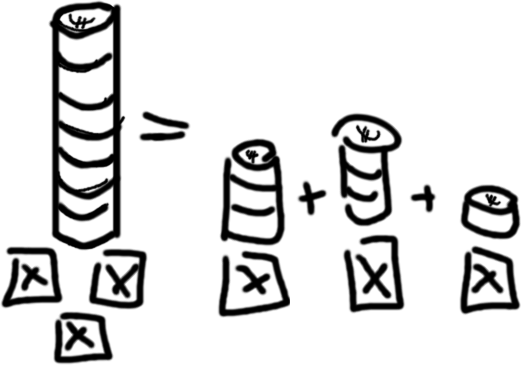
\includegraphics[height=2.5cm]{img/additive}
		\end{subfigure}
		\hfil
		\begin{subfigure}{36.5mm}
			\begin{overprint}
				\includegraphics<.(-2)|handout:0>[height=2.5cm]{img/submodular}%
				\includegraphics<.(-1)->[height=2.5cm]{img/submodular_full}%
			\end{overprint}
		\end{subfigure}
		\hfil
		\begin{subfigure}{28mm}
			\onslide<.->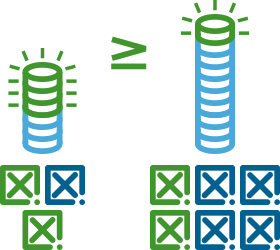
\includegraphics[height=2.5cm]{img/diminishingreturns}
		\end{subfigure}
	\end{figure}
\end{frame}





\subsection{Maximum Nash Social Welfare Problem}
\begin{frame}{Asymmetric Maximum Nash Social Welfare Problem}
	\pause
	\adjustfortopblock
	\begin{problem}<2->
		\begin{equation*}
			\alloc*[][] \overset{!}{=} \smashoperator{\argmax_{\alloc[][] \in \allallocs{\scriptstyle\agents\kern1pt}{\goods}}} \braces{ \NSW(\alloc[][]) }
			\onslide<4->{
				\qquad\text{with}\qquad
				\NSW(\alloc[][]) \coloneq \paren[\Big]{ \smashoperator{\prod_{i \in \agents}} \valuations[\alloc]^{\,\textstyle\weight} }{}^{\textstyle 1 / \sum_{i \in \agents} \weight}
			}
		\end{equation*}
		\begin{itemize}
			\item<2->
			\(\allallocs{\agents\kern1pt}{\goods}\): all possible allocations

			\item<3->
			\(\weight\): agent weight
		\end{itemize}
	\end{problem}
	\onslide<5->{The NSW strikes a middle ground between efficiency and fairness!}
	\begin{alertblock}<6->{}
		Is there an algorithm with an approximation factor \dots
		\begin{itemize}
			\item<8->
			\dots{} dependent on \(n\)?

			\item<9->
			\dots{} independent from \(m\)?
		\end{itemize}
		\def\svgwidth{3cm}
		\beamerimage<7-> at (13.5cm, 1.1cm) {\input{img/nvsm.pdf_tex}};
		\vspace{-0.75ex}
	\end{alertblock}
\end{frame}